International passenger traffic has been monitored to continuously increase over the years. Since air transport is one of the most convenient form of long distance transport among passengers, the above claim is indicated by the Airports Council International's Passenger Traffic Summary \footfullcite{aci_world_2019}. Despite the current shock due to the Covid-19 pandemic to the air transport industry, the aviation industry has shown resilience over the past decades and is predicted to recover and further grow by $ 4\% $ over the course of the next 20 years \footfullcite{Boeing2020} international border crossing points are forecasted to face more traffic than they already are. Implying the requirement for a solution to the Border control process to mitigate longer queues and waiting times, or the need to hire and train more personnel to conduct the task.
\par
Bio-metric passports are widely issued by more than 150 countries and regions, as of 2020 \footfullcite{ReadID2020}. Such passports contain a contactless smart chip that stores the passport holder's bio-metric information to authenticate his identity at passport control stations. The chips may contain one or more of the following bio-metric data: Iris, Fingerprint, and/or Facial features. In recent years, \gls{abc} systems, or E-Gates, started rolling out in airports leveraging the wide deployment of bio-metric passports. They intend to automate the process and improve the management and control of travel flows, serving passengers in a shorter time and reduce queues at airports. Resulting in benefits to the Aircraft operators, Airports, passengers, and Governments \cite{Angiolelli-meyer2015}.
\par
% types of E-gates
%- modules and services in the E-gate
Labati et al. \cite{labati2016biometric} represented two types of communication performed at an E-Gate: communication between systems interconnected within the E-Gate, and communication with External systems. Internally, an E-Gate is composed of 4 subsystems: \gls{das}, \gls{bvs}, \gls{csi}, and \gls{bgms}. Externally, the E-gate is part of a larger border control infrastructure. It communicates with external systems to query for additional information to verify the traveler's eligibility to be granted access to cross the border. An E-Gate can query the databases of the following external systems: \gls{vms}, \gls{rtp}, and \gls{eems}. Figure \ref{E-Gate-Architecture} from \cite{labati2016biometric} presents an illustrative overview of the E-Gate logical architecture. Essentially, the data transfer between the above systems, internally and externally, must be secure as it includes personal data, bio-metrics, and decision making information that affect a state's national security.
\begin{figure}[H]
	\centering
	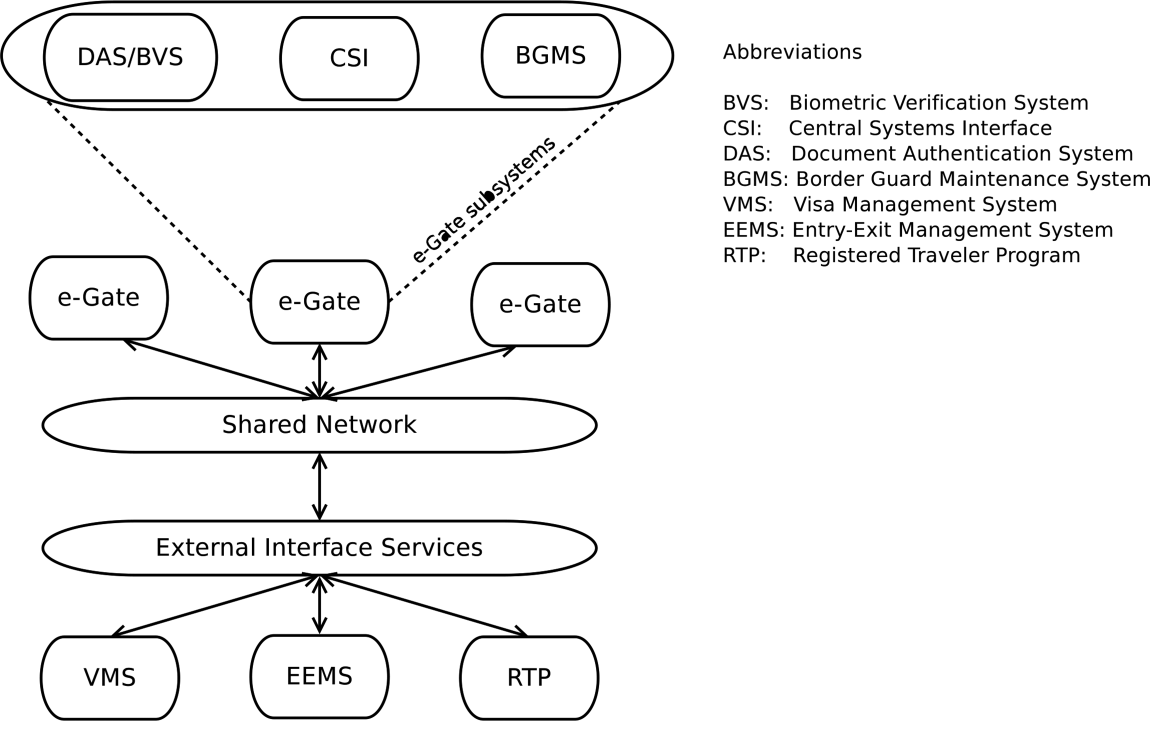
\includegraphics[scale=0.35]{Images/E-Gate-Architecture.png}
	\caption{ABC Logical Architecture overview \cite{labati2016biometric}}
	\label{E-Gate-Architecture}
\end{figure}

\par
The workflow of the ABC systems is similar to the one depicted in Figure \ref{workflow}. At first, a citizen starts by scanning his passport data page through the gate's scanner. The scanner communicates the image to the Border control system (BCS) which in turn runs its optical data recognition software to extract the data from the scanned data page and verify the document security features. Next, the E-Gate proceeds by reading the embedded electronic chip in the passport. Due to the sensitivity of the bio-metric data, they are not transferred. However, the non-sensitive data stored on the chip, which is equivalent to the data already scanned, is sent to the BCS to cross-check the passport data page. The citizen's facial features and bio-metrics are scanned by the E-Gate to authenticate the citizen against the chip's data. Finally, If the BCS verifies the passport, the E-Gate verifies the bio-metric features, and no match was found in the BCS's watchlists, then the citizen is allowed to pass the border checkpoint.

\begin{figure}[H]
	\centering
	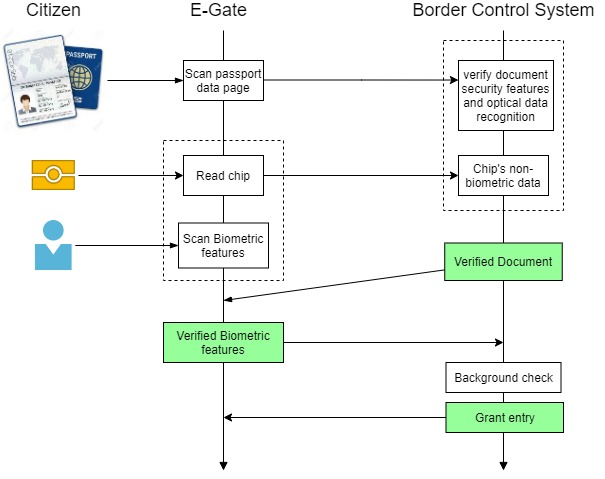
\includegraphics[scale=0.32]{Images/ABC.jpeg}
	\caption{Workflow of ABC.}
	\label{workflow}
\end{figure}
%attacks on E-Gates (facial recognition)